\documentclass[12pt,a4paper]{scrartcl}
\usepackage{ifpdf}
\usepackage[utf8]{inputenc}
\usepackage[ngerman]{babel}
\usepackage{amsmath}
\usepackage{amssymb}
\usepackage{fancyhdr}
\usepackage{listings}
\usepackage{color}
\usepackage{pdfpages}
\usepackage{stmaryrd}
\lstset{% general command to set parameter(s) 
basicstyle=\small	% print whole listing small
}

\renewcommand{\author}[1]{\newcommand{\printAuthor}{#1}}
\renewcommand{\title}[1]{\newcommand{\printTitle}{#1}}
\title{Serie 01}
\author{Johannes Hedtrich, Nikolaus Majewski}
\date{\today}

\pagestyle{fancy}
\fancyhead{}
\fancyfoot{}
\fancyhead[LO,LE]{\printAuthor}
\fancyhead[RO,RE]{\printTitle}
\fancyfoot[CO,CE]{\thepage}
 
\title{Serie 09}

\begin{document} 

  \section*{Aufgabe 9.3 Max-Flow}
  \textbf{Voraussetzung: } Sei der Graph wie in der Aufgabenstellung gegeben.
  
  \noindent
  \textbf{Behauptung: } Der maximale Fluss beträgt 31 Einheiten.
  
  \noindent
  \textbf{Beweis: }
  
  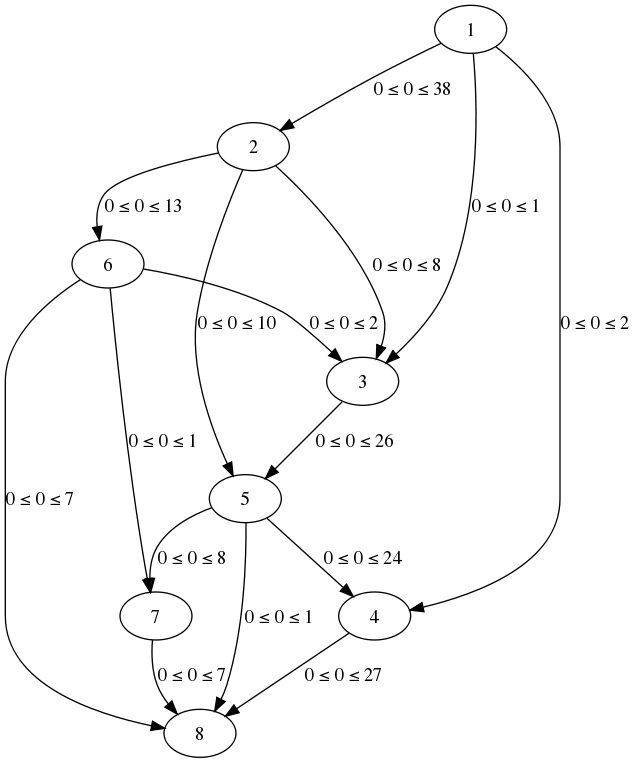
\includegraphics[width=0.45\textwidth]{img/0-graph.png}
  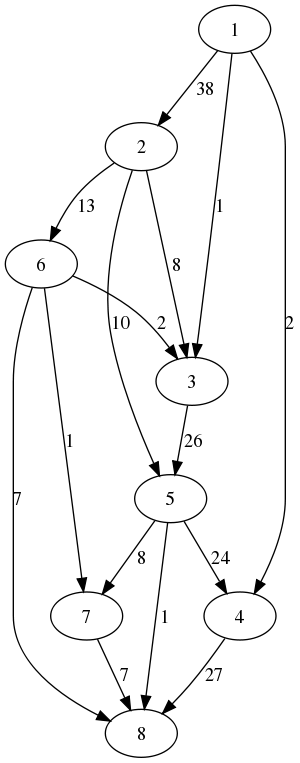
\includegraphics[height=0.6\textwidth]{img/0-res-graph.png}
  
  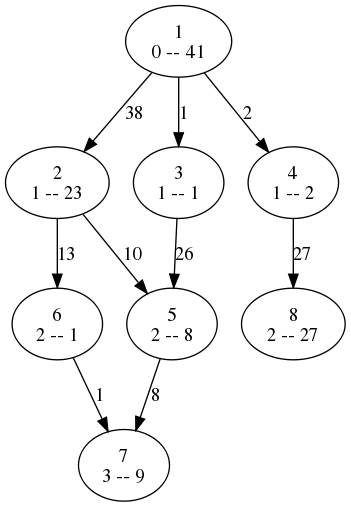
\includegraphics[width=0.45\textwidth]{img/0-level-graph.png}
  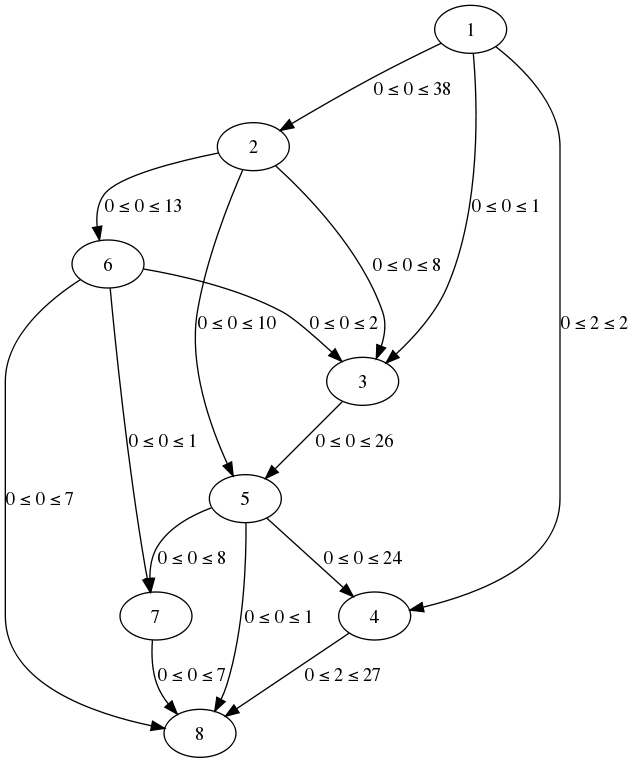
\includegraphics[width=0.45\textwidth]{img/1-graph.png}

  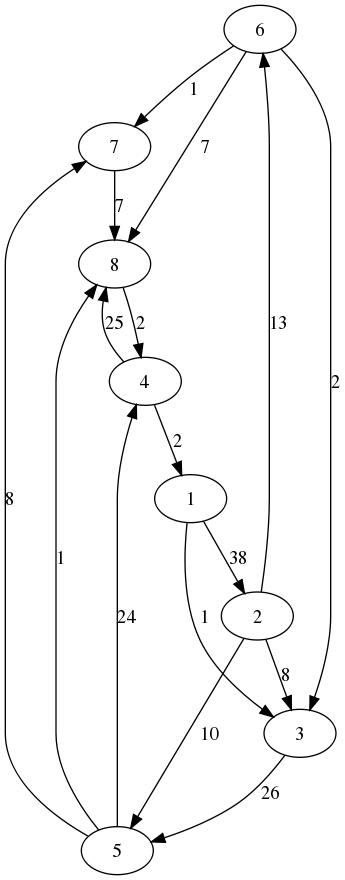
\includegraphics[height=0.6\textwidth]{img/1-res-graph.png}
  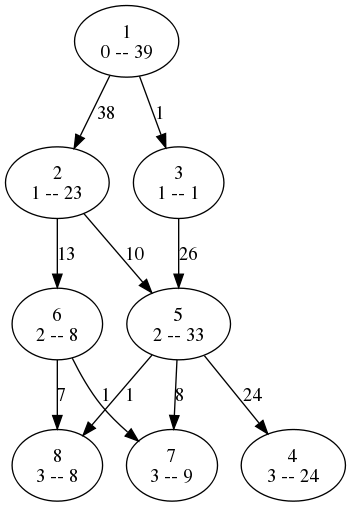
\includegraphics[width=0.45\textwidth]{img/1-level-graph.png}
  
  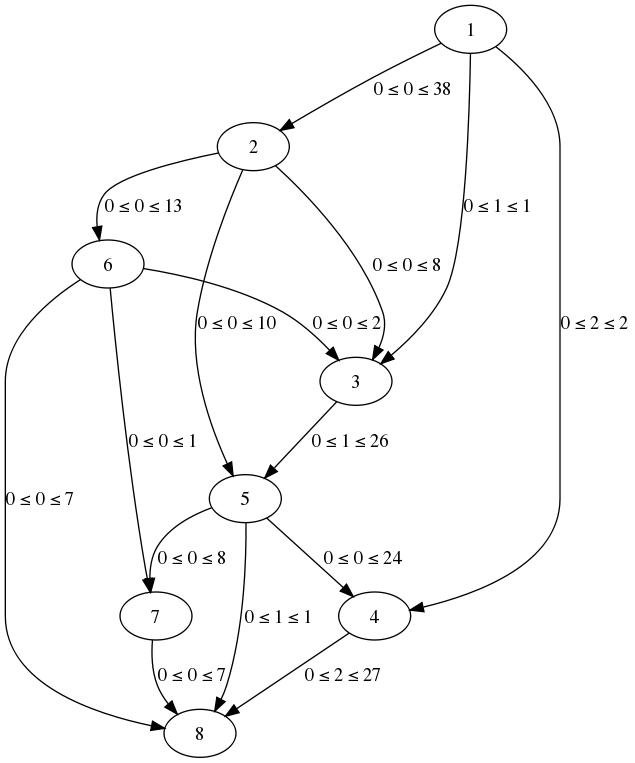
\includegraphics[width=0.45\textwidth]{img/2-graph.png}
  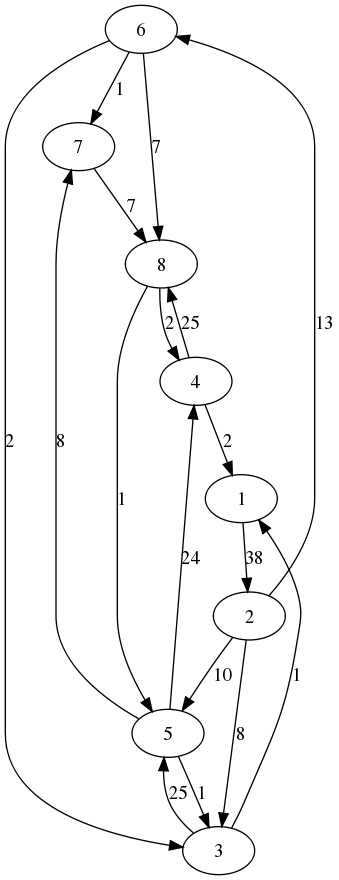
\includegraphics[height=0.6\textwidth]{img/2-res-graph.png}
  
  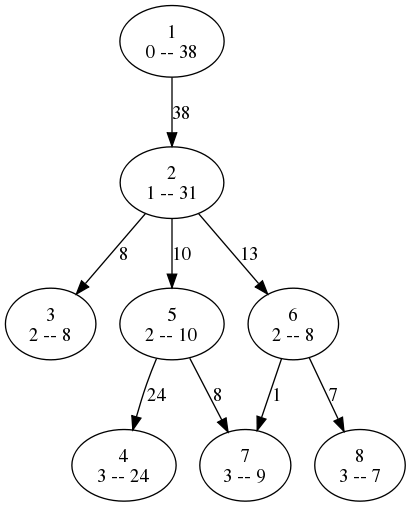
\includegraphics[width=0.45\textwidth]{img/2-level-graph.png}
  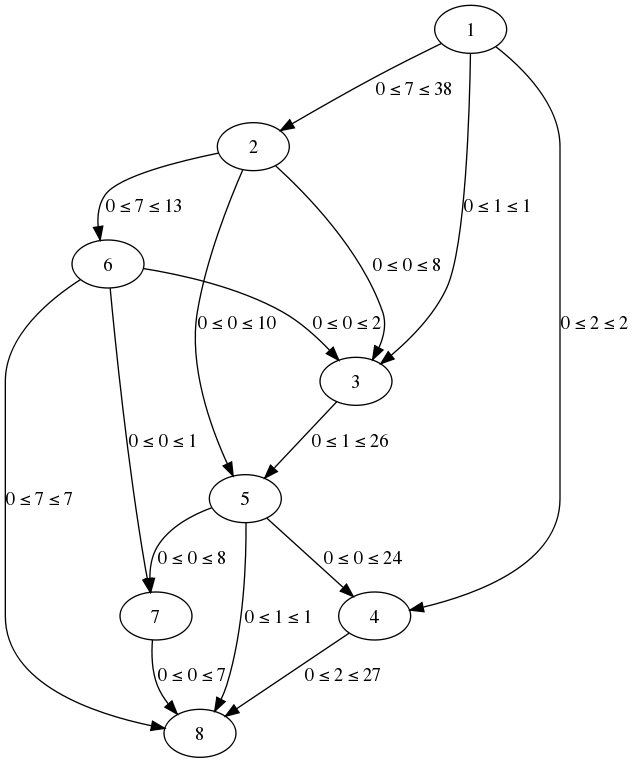
\includegraphics[width=0.45\textwidth]{img/3-graph.png}

  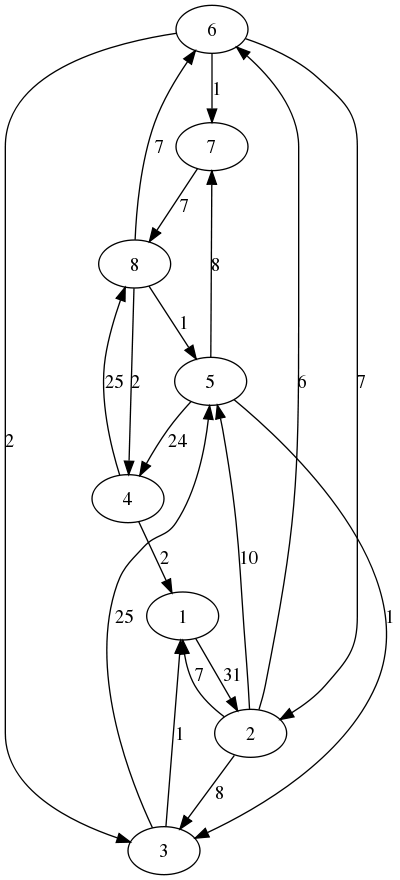
\includegraphics[height=0.9\textwidth]{img/3-res-graph.png}
  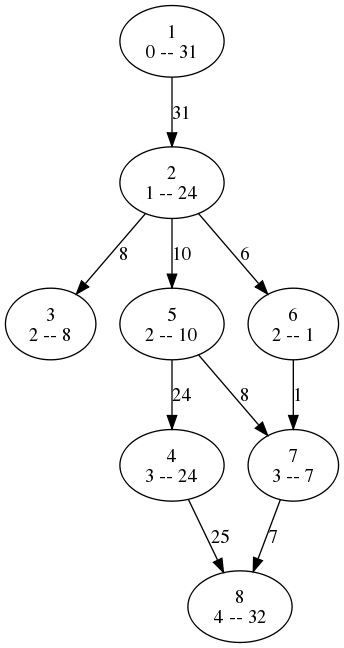
\includegraphics[height=0.9\textwidth]{img/3-level-graph.png}
  
  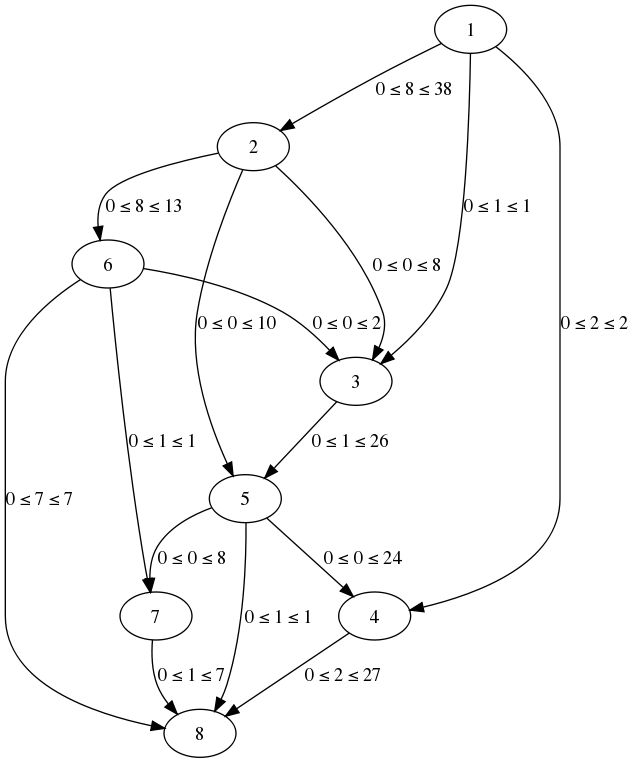
\includegraphics[width=0.5\textwidth]{img/4-graph.png}
  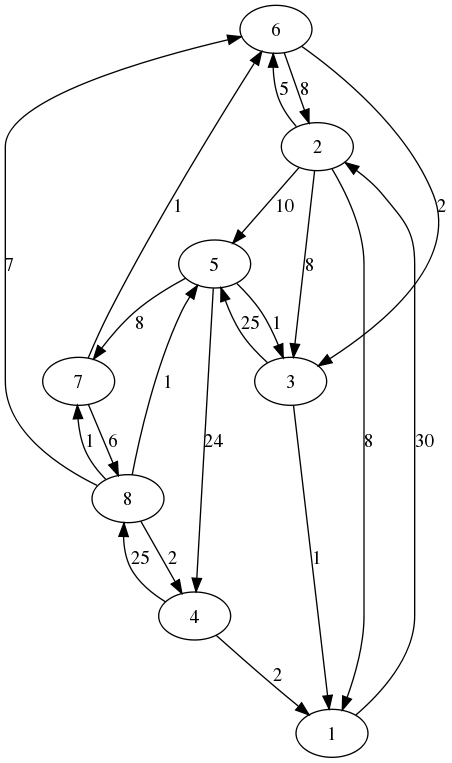
\includegraphics[height=0.6\textwidth]{img/4-res-graph.png}
  
  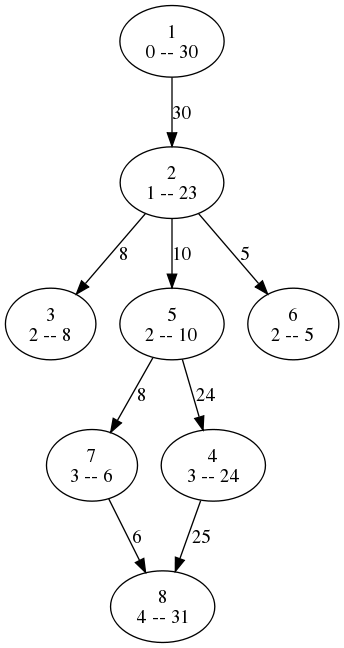
\includegraphics[width=0.45\textwidth]{img/4-level-graph.png}
  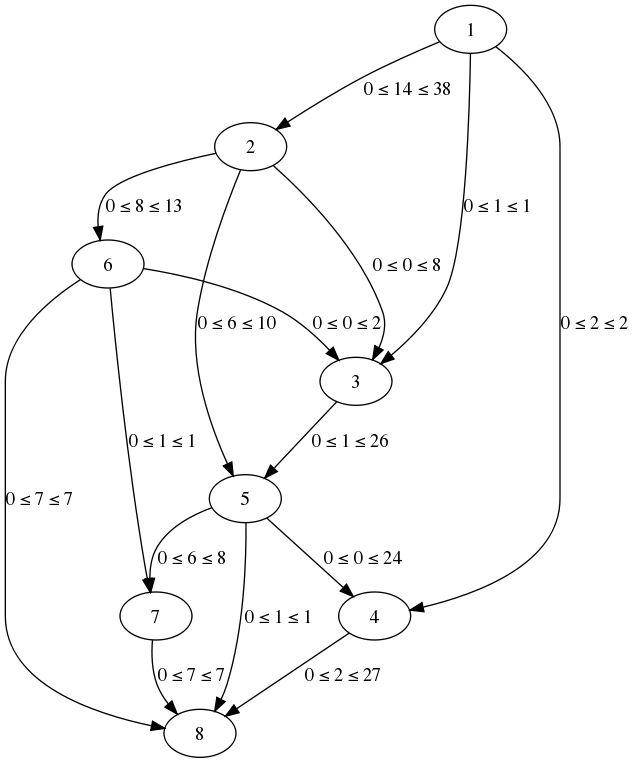
\includegraphics[width=0.45\textwidth]{img/5-graph.png}

  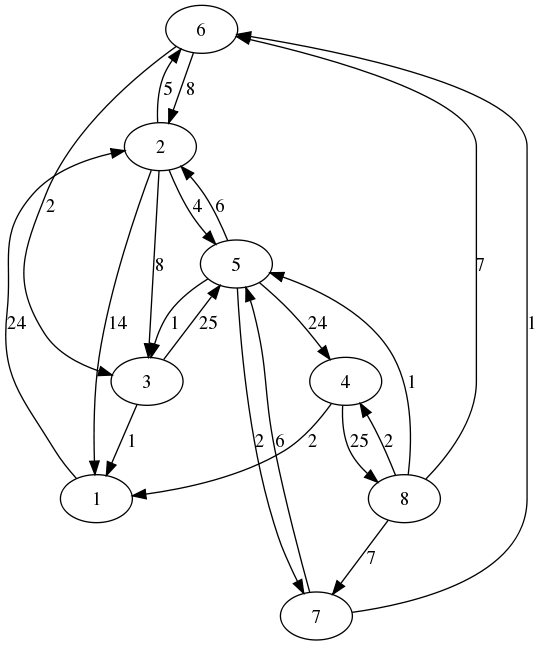
\includegraphics[width=0.45\textwidth]{img/5-res-graph.png}
  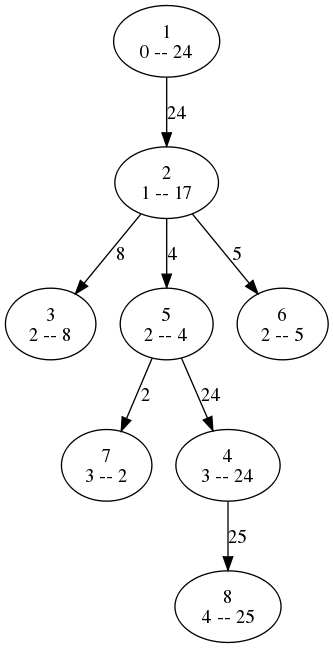
\includegraphics[height=0.6\textwidth]{img/5-level-graph.png}
  
  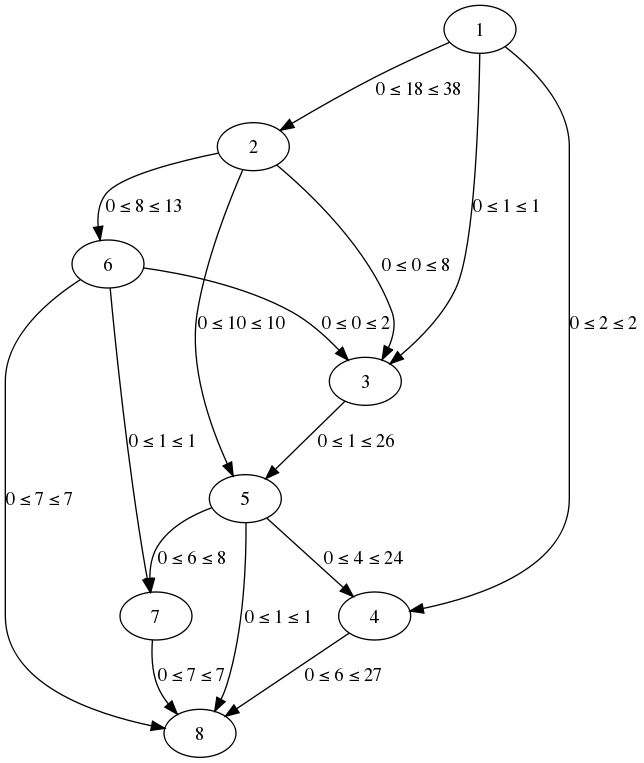
\includegraphics[width=0.45\textwidth]{img/6-graph.png}
  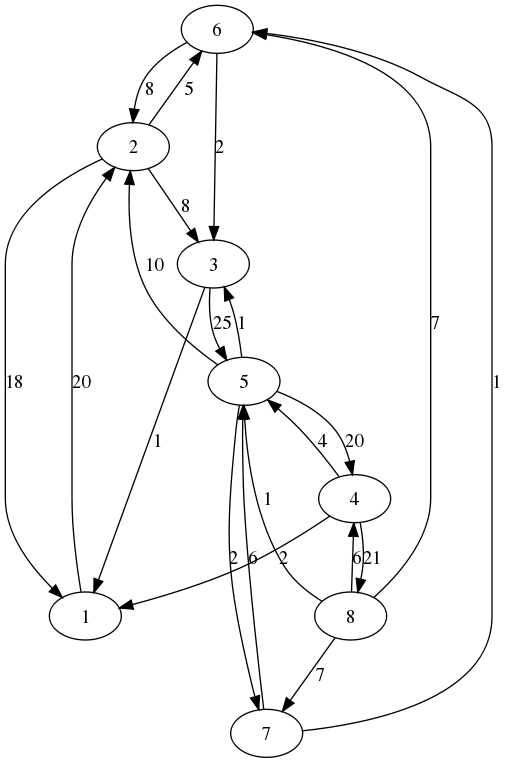
\includegraphics[height=0.6\textwidth]{img/6-res-graph.png}
  
  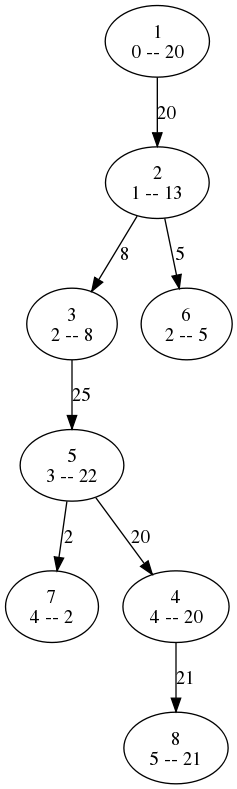
\includegraphics[height=0.6\textwidth]{img/6-level-graph.png}
  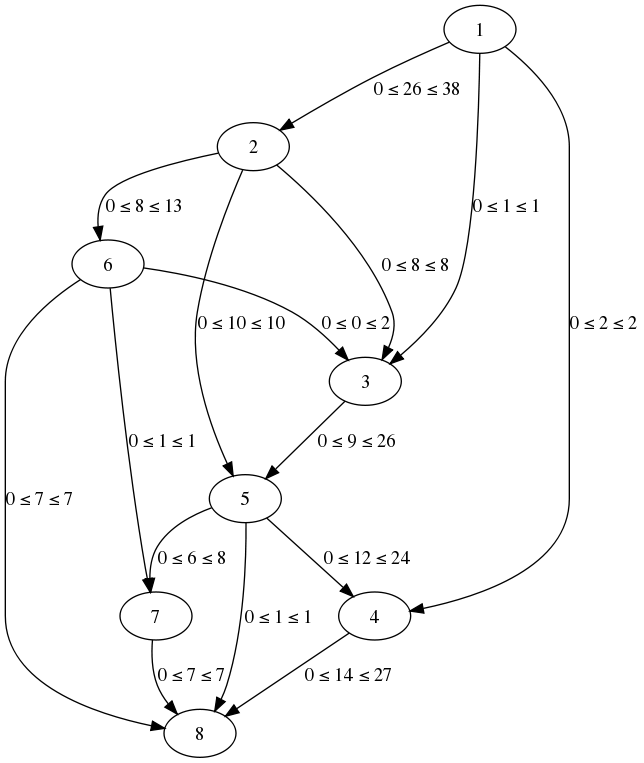
\includegraphics[width=0.45\textwidth]{img/7-graph.png}

  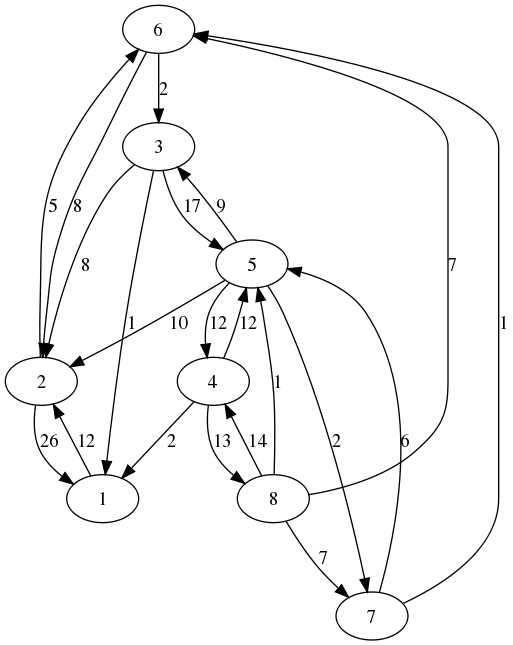
\includegraphics[width=0.45\textwidth]{img/7-res-graph.png}
  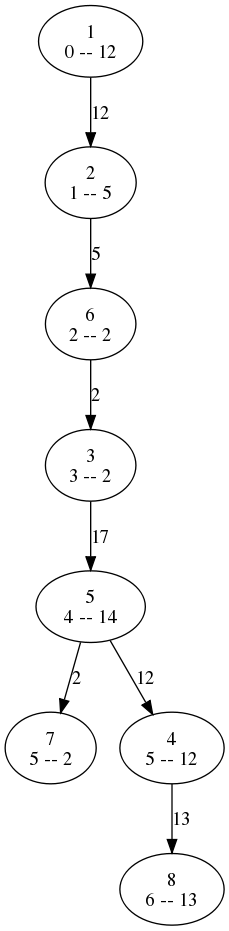
\includegraphics[height=0.6\textwidth]{img/7-level-graph.png}

  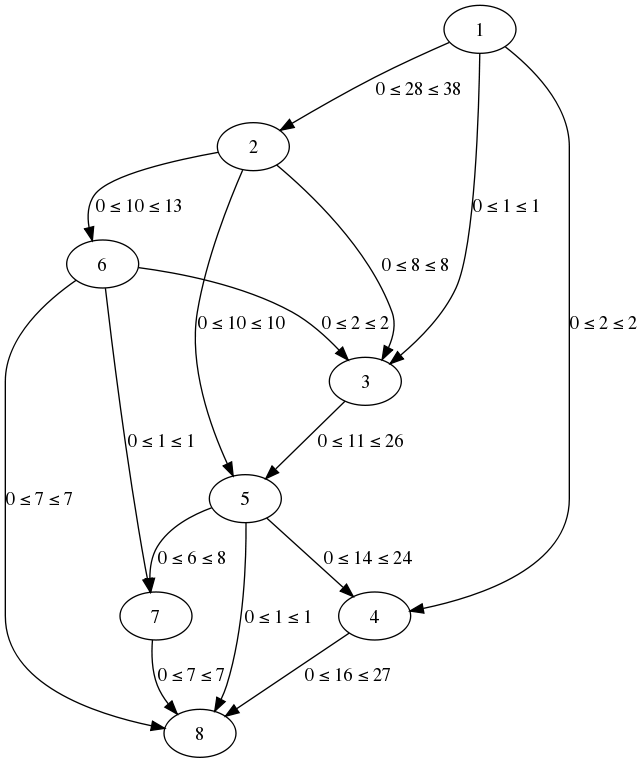
\includegraphics[width=0.45\textwidth]{img/8-graph.png}
  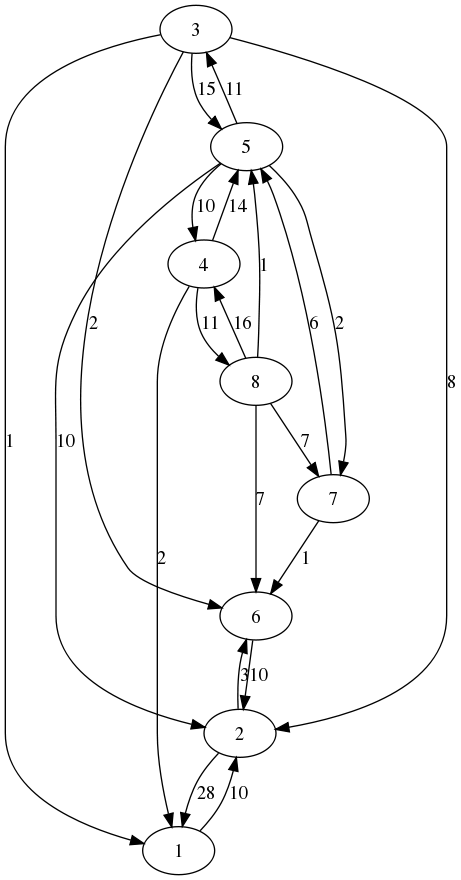
\includegraphics[height=0.6\textwidth]{img/8-res-graph.png}
  
  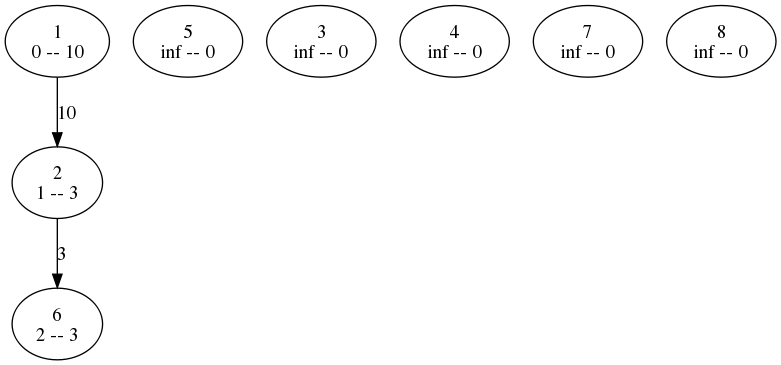
\includegraphics[width=0.7\textwidth]{img/8-level-graph.png}
  
\end{document}